% Created 2014-12-05 Fri 19:32
\documentclass[11pt]{article}
\usepackage[utf8]{inputenc}
\usepackage[T1]{fontenc}
\usepackage{fixltx2e}
\usepackage{graphicx}
\usepackage{longtable}
\usepackage{float}
\usepackage{wrapfig}
\usepackage{rotating}
\usepackage[normalem]{ulem}
\usepackage{amsmath}
\usepackage{textcomp}
\usepackage{marvosym}
\usepackage{wasysym}
\usepackage{amssymb}
\usepackage{hyperref}
\tolerance=1000
\author{Üstün Özgür}
\date{\today}
\title{Postgresql: Web Programcısı için Gündelik İpuçları \\ Postgres 2014 Türkiye}
\hypersetup{
  pdfkeywords={},
  pdfsubject={},
  pdfcreator={Emacs 24.4.1 (Org mode 8.2.10)}}
\begin{document}

\maketitle
\tableofcontents


\section{Giriş}
\label{sec-1}

Günümüzde pek çok web yazılım mimarisi MVC mimarisini kullanmakta. Java için
Spring, Ruby için Rails, Python için Django gibi. Bu mimarilerin genel bir
özelliği de ORM kullanımını popülerleştirmeleri. ORM işlerin çoğunu
kolaylaştırsa da programcı ile veritabanı arasında bir duvar
oluşturmakta. Halbuki bu yapılan web uygulamalarında temel amaç zaten verinin
saklanması, bu noktada veritabanının programcı tarafından dert edilmemesi
gereken bir araç olduğu kanısı baş ağrıtmakta.

Bu sunumda bir web programcısının bilmesi gereken Postgres kavramları ve
ipuçlarına değineceğim.

\section{SQL Bir Programlama Dilidir}
\label{sec-2}

SQL temelde relation denilen ilişkilere yönelik bir sorgulama dili olsa da
aslında ilk bakışta göründüğünden daha güçlü bir dil. Nasıldan çok neyi
istediğimizi söylediğimiz deklaratıf bir dil.


\subsection{Bir Programlama Dili Olarak SQL}
\label{sec-2-1}

\begin{itemize}
\item İlişkiler üzerinde operasyonlar
\item Genelde sütun bazında operasyonlar: Yüksek seviye fonksiyonlar
\item Yanlış bir tabir de olsa SQL için fonksiyonel diyebiliriz
\item Üç temel yüksek seviye fonksiyon: Map, Filter, Reduce
\item SQL hepsini sağlıyor.
\item Map \texttt{SELECT foo(x) from table};
\item foo fonksiyonunu bütün x değerleri için uygula
\item \texttt{SELECT foo(x) from table where predicate(x)} dediğimizde
\end{itemize}
filter'a denk şekilde bir predicate fonksiyonu uygular. (Predicate fonksiyon
boolean dönen fonksiyon)
\begin{itemize}
\item Eğer foo aggregate yapıda bir fonksiyon ise de reduce'a denktir diyebiliriz.
\end{itemize}


\subsection{Örnek: Faktoriyel Implementasyonu}
\label{sec-2-2}
\begin{verbatim}
select generate_series(1, 10);
select generate_series(1, 10, 2);
select 3 * 4;
select numeric_mul(3, 4);
create aggregate function product(numeric)
   (sfunc=numeric_mul, stype=numeric, initcond=1);
select product(x) from generate_series(1, 5) as x;
create function myfactorial(i numeric) returns integer as 'select product(x)
from generate_series(1, i::integer) as x;' language sql;
\end{verbatim}

Trivia: Postgresql'de kac tane fonksiyon vardir?

\begin{verbatim}
\df
\set ECHO_HIDDEN
\end{verbatim}

\subsection{psql}
\label{sec-2-3}

Postgresql için birçok GUİ client'i var, bunları kullanmak zaman zaman daha
kullanışlı olabilir; ancak psql aracını kullanmayı bilmek çok önemlidir. psql
aracının rahat kullanımı denemeler yapmayı kolaylaştıracak ve SQL pratiği yapmak
açısından faydalı olacaktır.

Önemli psql komutları: En önemli psql komutları \texttt{\textbackslash{}h} ve \texttt{\textbackslash{}?}'dır. Bu iki komut ile
yapılacak her şey ile ilgili bilgi almak mümkün. \texttt{\textbackslash{}h} ile sql komutları hakkında
bilgi alınırken \texttt{\textbackslash{}?} ile psql'e özel komutlar hakkında bilgi alınabilir.


\begin{verbatim}
\h
\h CREATE
\h CREATE TABLE
\h ALTER TRİGGER
\end{verbatim}

Psql'a ait özel komutlar $\backslash$ ile başlar ve bunlarla veritabanımız hakkında hızlıca
bilgi alabiliriz.

\begin{verbatim}
\l
\d
\d+
\df
\dft
\e
\o
\H
\! make_pretty_table foo.html
\end{verbatim}


Kısa bir dipnot: \texttt{\textasciitilde{}/.psqlrc}'ye koyacağımız komutlar başlangıçta
çalıştırılacaktır.

\begin{verbatim}
\x auto
\timing
\end{verbatim}


\section{Performans ipuçlarıÖ}
\label{sec-3}

Sayfalarınızda toplamda kaç tane SQL sorgusunun gösteren bir araç
kullanın. Örneğin Django için django-debug-toolbar.

psql'de \texttt{\textbackslash{}timing} kullanımı, \texttt{ANALYZE} ve \texttt{EXPLAIN ANALYZE} komutu ve buna göre index
ekleme.

ORM'lerde olabilecek en büyük sorun N+1 sorguları. Örneğin N tane soru
göstereceksiniz, bu soruları soran kişinin de ismini göstereceksiniz. N+1
tehlikesine çok müsait. Django için \texttt{select\_related} ve \texttt{prefetch\_related} bunları
azaltacaktır.

Bağlantı havuzu: Bağlantıların kurulması çok fazla zaman alabilir. Mutlaka
pgbouncer gibi bir bağlantı havuzu sağlayın. Kurulması oldukça kolay.

pgtüne uygulaması: Postgres'in default konfigürasyonu oldukça muhafazakar bir
şekilde hazırlanmıştır, bunu makineye göre optimize etmek için
\url{https://github.com/gregs1104/pgtune} ve Web versiyonu
\url{http://pgtune.leopard.in.ua/}

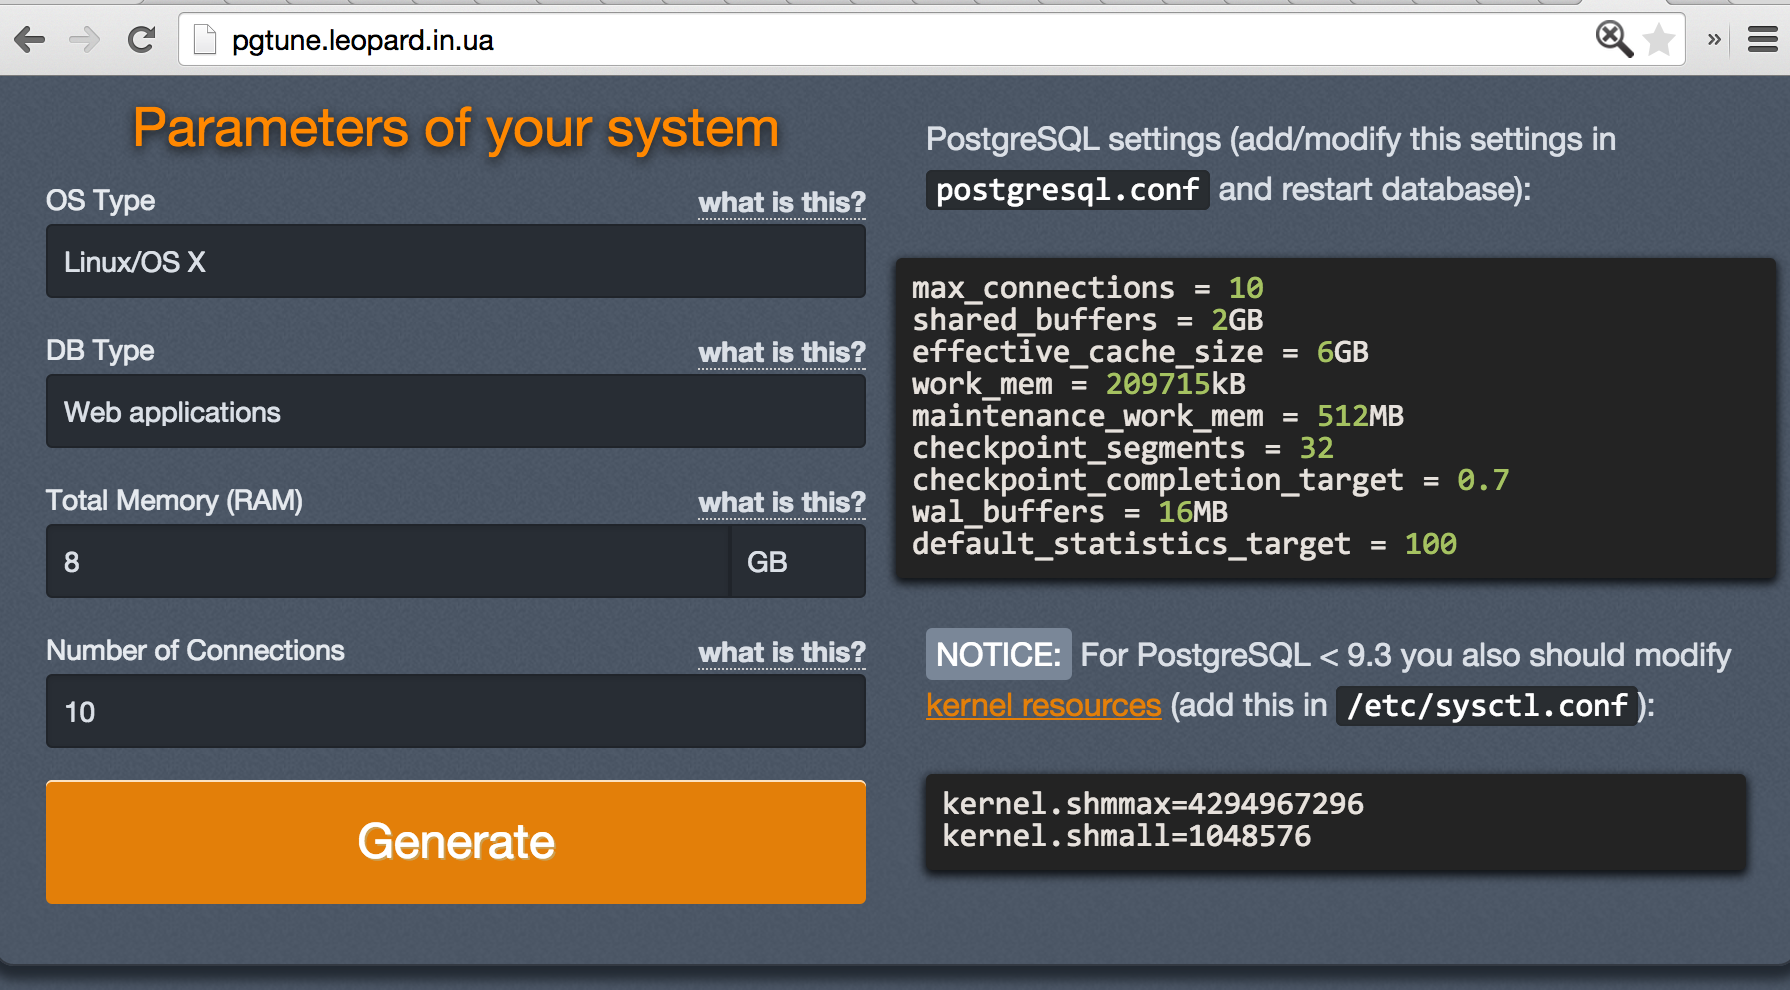
\includegraphics[width=.9\linewidth]{./pgtune.png}

Sessionları veritabanında tutmak yerine redis gibi ikinci bir araçta
tutabilirsiniz.

Pghero: \url{https://github.com/ankane/pghero}

\begin{itemize}
\item SELECT * FROM pghero$_{\text{missing}}$$_{\text{indexes}}$;
\item SELECT * FROM pghero$_{\text{relation}}$$_{\text{sizes}}$;
\item SELECT pghero$_{\text{index}}$$_{\text{hit}}$$_{\text{rate}}$();
\item SELECT * FROM pghero$_{\text{unused}}$$_{\text{indexes}}$;
\end{itemize}

Monitoring için NewRelic ya da AppNeta gibi araçlar da production esnasında performans
sorunlarını takip etmek için kullanılabilir. Bu araçların kurulumu oldukça
zahmetsiz.


\section{Yedekler}
\label{sec-4}

En azından \texttt{pg\_dump} ile günlük backuplar alın ve başka bir makineye (S3 vs.)
gönderin.

Projenin kritikliğine göre streaming replication yapabilirsiniz, son
Postgres sürümlerinde bu oldukça kolaylaştı. Bu konuda Josh Berkus'un "Ten
Minutes to Replication" sunumunu
izleyin. \url{http://www.youtube.com/watch?v=BD7i9QImqic}
% Emacs 24.4.1 (Org mode 8.2.10)
\end{document}
